% 图 25.1 —— 由 `checks/emit_hand.py` 自动拼出（probe 精测 + prims2 图元分解）
%%
% ⚠ 这是**稿子不是成品**：跑 `checks/checkhand.py 25.1` 看指标 + 看叠合图。
%%
%% ⚠ 待核：
%   · 本图 probe 报出阴影族 1 个 —— **本脚本不生成阴影**（要照原书手写）；prims2 的 strokes 里可能含阴影线，核对时留意别画重
%   · 可疑字形 1 项（空心圈 ⊙ 常被认成字母 o）—— 见文件末
%%
\documentclass[12pt]{standalone}
\usepackage{fontspec}
\setsansfont{Arial}
\newfontfamily\mfallback{DejaVu Sans}
\usepackage{tikz}
\usetikzlibrary{arrows.meta}
\begin{document}
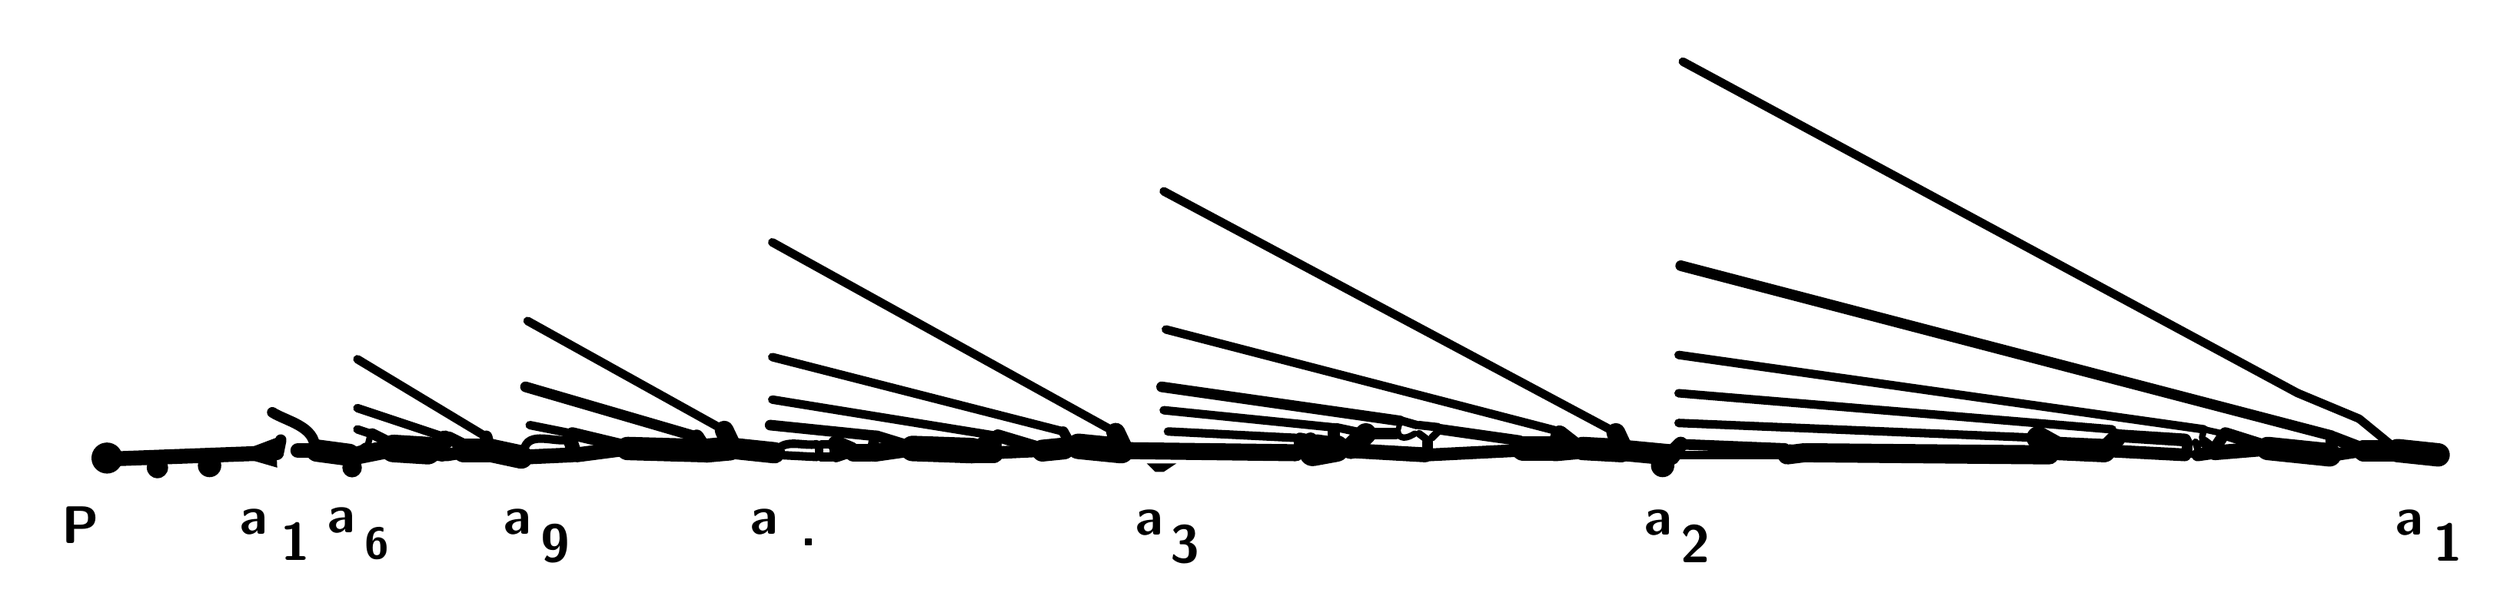
\begin{tikzpicture}[x=1pt, y=-1pt, line width=4.0pt, line cap=round, line join=round]

  %% ════ 填充区（prims2 的 fills）════
  \fill (529.0,208.0) -- (533.0,212.0) -- (537.0,212.0) -- (543.0,208.0) -- cycle;

  %% ════ 直线段（prims2 的 strokes）════
  \draw[line width=4.0pt] (374.0,205.0) -- (355.0,204.0);
  \draw[line width=5.0pt] (383.0,205.0) -- (389.0,203.0);
  \draw[line width=5.3pt] (121.0,202.0) -- (122.0,197.0);
  \draw[line width=7.0pt] (130.0,202.0) -- (137.0,202.0);
  \draw[line width=4.0pt] (539.0,193.0) -- (599.0,196.0);
  \draw[line width=6.0pt] (458.0,203.0) -- (479.0,202.0);
  \draw[line width=5.1pt] (1026.0,198.0) -- (1030.0,201.0);
  \draw[line width=4.0pt] (779.0,189.0) -- (948.0,196.0);
  \draw[line width=10.9pt] (948.0,196.0) -- (957.0,201.0);
  \draw[line width=10.3pt] (480.0,202.0) -- (490.0,201.0);
  \draw[line width=6.0pt] (617.0,198.0) -- (617.0,192.0);
  \draw[line width=6.0pt] (459.0,195.0) -- (479.0,201.0);
  \draw[line width=7.0pt] (1055.0,201.0) -- (1031.0,203.0);
  \draw[line width=10.0pt] (754.0,202.0) -- (775.0,204.0);
  \draw[line width=7.1pt] (601.0,202.0) -- (606.0,197.0);
  \draw[line width=6.0pt] (206.0,203.0) -- (200.0,204.0);
  \draw[line width=4.0pt] (781.0,19.0) -- (1069.9,174.9);
  \draw[line width=4.0pt] (1069.9,174.9) -- (1098.9,187.0);
  \draw[line width=4.0pt] (1098.9,187.0) -- (1116.0,201.0);
  \draw[line width=11.0pt] (219.0,202.0) -- (208.0,202.0);
  \draw[line width=3.4pt] (1023.0,201.0) -- (1022.0,198.0);
  % （略）线段 (129.0,201.0)-(123.0,196.0) 线宽8.5 —— 是箭头头那一坨，已由箭头头代替
  \draw[line width=2.5pt] (648.0,189.0) -- (647.0,193.0);
  \draw[line width=3.5pt] (661.0,197.0) -- (657.0,194.0);
  \draw[line width=9.0pt] (839.0,203.0) -- (953.2,204.0);
  \draw[line width=5.0pt] (953.2,204.0) -- (957.0,201.0);
  \draw[line width=6.3pt] (192.0,203.0) -- (198.0,204.0);
  \draw[line width=6.0pt] (1086.0,203.0) -- (1086.0,197.0);
  \draw[line width=9.6pt] (448.0,203.0) -- (457.0,203.0);
  \draw[line width=8.9pt] (753.0,201.0) -- (749.5,193.5);
  \draw[line width=4.0pt] (749.5,193.5) -- (537.0,80.0);
  \draw[line width=7.0pt] (660.0,204.0) -- (625.0,202.0);
  \draw[line width=6.0pt] (1087.0,204.0) -- (1100.0,202.0);
  \draw[line width=11.0pt] (1117.0,202.0) -- (1136.0,204.0);
  \draw[line width=3.0pt] (163.0,199.0) -- (164.0,195.0);
  \draw[line width=6.0pt] (618.0,201.0) -- (624.0,201.0);
  \draw[line width=12.6pt] (618.0,201.0) -- (607.0,203.0);
  \draw[line width=4.0pt] (458.0,195.0) -- (353.0,178.0);
  \draw[line width=5.0pt] (352.0,190.0) -- (401.0,195.0);
  \draw[line width=2.0pt] (164.0,200.0) -- (167.0,199.0);
  \draw[line width=13.0pt] (191.0,202.0) -- (175.0,201.0);
  \draw[line width=12.0pt] (447.0,202.0) -- (419.0,201.0);
  \draw[line width=10.0pt] (721.0,202.0) -- (732.0,201.0);
  \draw[line width=5.5pt] (1031.0,201.0) -- (1035.0,195.0);
  \draw[line width=6.0pt] (1023.0,204.0) -- (1030.0,203.0);
  \draw[line width=5.0pt] (667.0,192.0) -- (704.3,197.3);
  \draw[line width=3.0pt] (704.3,197.3) -- (705.0,200.0);
  \draw[line width=11.0pt] (734.0,201.0) -- (752.0,202.0);
  \draw[line width=4.0pt] (239.0,190.0) -- (259.0,194.0);
  \draw[line width=10.0pt] (1116.0,202.0) -- (1101.0,202.0);
  \draw[line width=5.0pt] (1086.0,195.0) -- (780.0,115.0);
  \draw[line width=7.0pt] (259.0,204.0) -- (237.0,205.0);
  \draw[line width=6.6pt] (453.0,198.0) -- (448.0,202.0);
  \draw[line width=11.5pt] (720.0,201.0) -- (706.0,201.0);
  \draw[line width=6.0pt] (284.0,200.0) -- (259.0,194.0);
  \draw[line width=3.7pt] (702.0,202.0) -- (703.0,201.0);
  \draw[line width=6.0pt] (702.0,202.0) -- (662.0,204.0);
  \draw[line width=11.0pt] (320.0,202.0) -- (285.0,201.0);
  \draw[line width=7.1pt] (775.0,204.0) -- (780.0,199.0);
  \draw[line width=5.0pt] (780.0,199.0) -- (829.0,201.0);
  \draw[line width=4.0pt] (775.0,204.0) -- (829.0,204.0);
  \draw[line width=3.0pt] (1022.0,204.0) -- (1019.0,204.0);
  \draw[line width=8.5pt] (401.0,203.0) -- (415.0,201.0);
  \draw[line width=4.0pt] (375.0,204.0) -- (375.0,200.0);
  \draw[line width=4.0pt] (353.0,158.0) -- (489.8,193.0);
  \draw[line width=4.8pt] (489.8,193.0) -- (492.0,197.0);
  \draw[line width=5.0pt] (402.0,195.0) -- (415.0,199.0);
  \draw[line width=11.3pt] (333.0,201.0) -- (322.0,202.0);
  \draw[line width=4.0pt] (381.0,199.0) -- (376.0,199.0);
  \draw[line width=4.0pt] (600.0,197.0) -- (600.0,201.0);
  \draw[line width=5.0pt] (724.0,193.0) -- (733.0,200.0);
  \draw[line width=4.0pt] (382.0,200.0) -- (382.0,204.0);
  \draw[line width=6.0pt] (1017.0,204.0) -- (979.0,202.0);
  \draw[line width=11.0pt] (957.0,201.0) -- (979.0,202.0);
  \draw[line width=5.0pt] (661.0,203.0) -- (661.0,198.0);
  \draw[line width=4.0pt] (779.0,157.0) -- (1026.0,192.0);
  \draw[line width=4.0pt] (831.0,201.0) -- (838.0,202.0);
  \draw[line width=10.5pt] (139.0,202.0) -- (154.0,204.0);
  \draw[line width=8.0pt] (391.0,203.0) -- (399.0,203.0);
  % （略）线段 (121.0,203.0)-(129.0,202.0) 线宽9.0 —— 是箭头头那一坨，已由箭头头代替
  \draw[line width=8.9pt] (199.0,197.0) -- (192.0,202.0);
  \draw[line width=8.5pt] (985.0,196.0) -- (979.0,202.0);
  \draw[line width=4.0pt] (723.0,193.0) -- (538.0,145.0);
  \draw[line width=6.0pt] (1100.0,201.0) -- (1087.0,196.0);
  \draw[line width=8.2pt] (390.0,202.0) -- (383.0,199.0);
  \draw[line width=8.5pt] (174.0,201.0) -- (159.0,204.0);
  \draw[line width=4.0pt] (618.0,191.0) -- (632.0,194.0);
  \draw[line width=10.0pt] (354.0,203.0) -- (335.0,201.0);
  \draw[line width=4.7pt] (601.0,203.0) -- (605.0,203.0);
  \draw[line width=4.0pt] (649.0,188.0) -- (656.0,190.0);
  \draw[line width=4.0pt] (353.0,104.0) -- (514.4,193.4);
  \draw[line width=8.9pt] (514.4,193.4) -- (518.0,201.0);
  \draw[line width=5.5pt] (646.0,194.0) -- (632.0,194.0);
  \draw[line width=5.0pt] (171.0,197.0) -- (165.0,194.0);
  \draw[line width=9.9pt] (632.0,194.0) -- (625.0,201.0);
  \draw[line width=6.0pt] (458.0,196.0) -- (458.0,202.0);
  \draw[line width=8.0pt] (519.0,202.0) -- (599.0,203.0);
  \draw[line width=4.0pt] (158.0,159.0) -- (218.5,195.5);
  \draw[line width=5.9pt] (218.5,195.5) -- (220.0,201.0);
  \draw[line width=4.0pt] (381.0,205.0) -- (376.0,205.0);
  \draw[line width=9.0pt] (838.0,203.0) -- (830.0,204.0);
  \draw[line width=6.0pt] (1036.0,194.0) -- (1055.0,200.0);
  \draw[line width=4.0pt] (657.0,190.0) -- (666.0,191.0);
  \draw[line width=8.9pt] (334.0,200.0) -- (330.4,192.4);
  \draw[line width=4.0pt] (330.4,192.4) -- (238.0,141.0);
  \draw[line width=7.3pt] (616.0,199.0) -- (609.0,198.0);
  \draw[line width=6.0pt] (207.0,199.0) -- (201.0,196.0);
  \draw[line width=4.0pt] (616.0,191.0) -- (537.0,183.0);
  \draw[line width=3.0pt] (199.0,203.0) -- (200.0,198.0);
  \draw[line width=3.0pt] (1035.0,194.0) -- (1026.0,192.0);
  \draw[line width=11.0pt] (1085.0,204.0) -- (1056.0,201.0);
  \draw[line width=11.0pt] (221.0,202.0) -- (235.0,205.0);
  \draw[line width=3.5pt] (663.0,196.0) -- (666.0,193.0);
  \draw[line width=3.0pt] (985.0,194.0) -- (982.8,192.0);
  \draw[line width=4.0pt] (982.8,192.0) -- (779.0,175.0);
  \draw[line width=3.8pt] (162.0,200.0) -- (159.0,202.0);
  \draw[line width=4.0pt] (158.0,192.0) -- (164.0,194.0);
  \draw[line width=6.0pt] (986.0,195.0) -- (1017.0,197.0);
  \draw[line width=6.7pt] (258.0,197.0) -- (260.0,203.0);
  \draw[line width=5.0pt] (401.0,196.0) -- (400.0,202.0);
  \draw[line width=7.0pt] (261.0,204.0) -- (284.0,201.0);
  \draw[line width=7.7pt] (723.0,194.0) -- (721.0,201.0);
  \draw[line width=3.0pt] (1025.0,196.0) -- (1026.0,192.0);
  \draw[line width=12.0pt] (497.0,200.0) -- (517.0,202.0);
  \draw[line width=7.0pt] (120.0,203.0) -- (40.0,206.0);
  \fill (119.7,196.0) -- (120.3,210.0) -- (99.0,203.8) -- cycle;
  \draw[line width=5.0pt] (536.0,172.0) -- (648.0,188.0);
  \draw[line width=5.0pt] (1018.0,203.0) -- (1018.0,198.0);
  \draw[line width=6.8pt] (321.0,201.0) -- (317.5,195.5);
  \draw[line width=5.0pt] (317.5,195.5) -- (237.0,172.0);
  \draw[line width=5.0pt] (606.0,197.0) -- (601.0,196.0);
  \draw[line width=4.0pt] (158.0,182.0) -- (200.0,196.0);

  %% ════ 曲线（prims2 的 curves —— 三段式，坐标同为 (y,x)）════
  \draw[line width=3.0pt] (647.0,194.0) .. controls (648.9,197.4) and (652.7,195.4) .. (655.0,194.0);
  \draw[line width=4.0pt] (257.0,197.0) .. controls (249.0,198.1) and (236.5,191.8) .. (236.0,204.0);
  \draw[line width=5.0pt] (138.0,201.0) .. controls (138.1,190.5) and (124.9,188.3) .. (118.0,184.0);
  \draw[line width=4.0pt] (355.0,202.0) .. controls (359.4,196.3) and (367.7,200.1) .. (374.0,199.0);

  %% ════ 实心点 ════
  \fill (40.3,205.5) circle (7.3);
  \fill (88.5,209.0) circle (5.5);
  % （略）(115.0,208.5) r=6.0 落在箭头头上 —— 已由箭头头代替
  \fill (155.5,210.0) circle (4.6);
  \fill (771.5,209.0) circle (5.5);
  \fill (64.0,210.0) circle (5.0);

  %% ════ 标签（probe 直接给的 \node 行）════
  %% ⚠ 全部补了 fill=white：文字在最上层，否则与曲线交叉干扰
     \node[anchor=center,inner sep=0pt,fill=white,font=\fontsize{29.2}{36.4}\selectfont] at (27.9,237.0) {\textsf{\textbf{\textit{P}}}};   % box(17,225,18,22)
     \node[anchor=center,inner sep=0pt,fill=white,font=\fontsize{31.0}{38.7}\selectfont] at (150.5,235.0) {\textsf{\textbf{\textit{a}}}};   % box(142,225,15,17)
     \node[anchor=center,inner sep=0pt,fill=white,font=\fontsize{30.0}{37.6}\selectfont] at (109.5,235.5) {\textsf{\textbf{\textit{a}}}};   % box(101,226,15,16)
     \node[anchor=center,inner sep=0pt,fill=white,font=\fontsize{30.0}{37.6}\selectfont] at (233.5,235.5) {\textsf{\textbf{\textit{a}}}};   % box(225,226,15,16)
     \node[anchor=center,inner sep=0pt,fill=white,font=\fontsize{30.0}{37.6}\selectfont] at (349.5,235.5) {\textsf{\textbf{\textit{a}}}};   % box(341,226,15,16)
     \node[anchor=center,inner sep=0pt,fill=white,font=\fontsize{31.0}{38.7}\selectfont] at (530.5,236.0) {\textsf{\textbf{\textit{a}}}};   % box(522,226,15,17)
     \node[anchor=center,inner sep=0pt,fill=white,font=\fontsize{31.0}{38.7}\selectfont] at (769.5,236.0) {\textsf{\textbf{\textit{a}}}};   % box(761,226,15,17)
     \node[anchor=center,inner sep=0pt,fill=white,font=\fontsize{31.0}{38.7}\selectfont] at (1122.5,236.0) {\textsf{\textbf{\textit{a}}}};   % box(1114,226,15,17)
     \node[anchor=center,inner sep=0pt,fill=white,font=\fontsize{28.7}{35.9}\selectfont] at (128.8,245.0) {\textsf{\textbf{1}}};   % box(120,236,11,17)
     \node[anchor=center,inner sep=0pt,fill=white,font=\fontsize{24.1}{30.1}\selectfont] at (250.9,245.6) {\textsf{\textbf{9}}};   % box(244,236,11,18)
     \node[anchor=center,inner sep=0pt,fill=white,font=\fontsize{60.1}{75.1}\selectfont] at (370.0,245.0) {\textsf{\textbf{.}}};   % box(360,236,11,17)
     \node[anchor=center,inner sep=0pt,fill=white,font=\fontsize{22.7}{28.3}\selectfont] at (167.1,245.6) {\textsf{\textbf{6}}};   % box(161,237,11,16)
     \node[anchor=center,inner sep=0pt,fill=white,font=\fontsize{23.0}{28.7}\selectfont] at (546.9,246.1) {\textsf{\textbf{3}}};   % box(541,237,11,17)
     \node[anchor=center,inner sep=0pt,fill=white,font=\fontsize{23.6}{29.6}\selectfont] at (787.1,245.9) {\textsf{\textbf{2}}};   % box(781,237,11,17)
     \node[anchor=center,inner sep=0pt,fill=white,font=\fontsize{23.7}{29.7}\selectfont] at (1140.8,245.4) {\textsf{\textbf{1}}};   % box(1134,237,8,16)

  % 钉死画布：否则超出的图元/控制点会把页面撑大，1:1 回比就失准
  \pgfresetboundingbox
  \path[use as bounding box] (0,0) rectangle (1155,265);
\end{tikzpicture}
\end{document}

% ⚠ 待核清单（probe 拿不准，人眼过一遍）：
%   · 未识别/跳过：⑤ 跳过/未识别的字形
